\section{Camera projective model}

A pinhole camera follows a perspective projection model that is inherently nonlinear, neither shape-preserving nor length-ratio preserving.
Despite this, it maintains the collinearity property: collinear points in the 3D scene are projected onto collinear points in the 2D image.
This implies a linear transformation between homogeneous coordinates, though the mapping is not invertible due to the loss of one dimension when capturing the image.

A 3D point $\mathbf{X}$ in homogeneous coordinates is projected onto an image point $\mathbf{u}$ through the camera projection matrix $\mathbf{P}$:
\[\mathbf{u}=\mathbf{PX}=\begin{bmatrix} \mathbf{M} & \mathbf{m} \end{bmatrix}\mathbf{X}\]
The back-projection of an image point $\mathbf{u}$ through a camera with projection matrix $\mathbf{P}=\begin{bmatrix} \mathbf{M} & \mathbf{m} \end{bmatrix}$ forms a straight line passing through the camera center $\mathbf{O}=\text{RNS}(\mathbf{P})$, with direction given by: $\mathbf{d}=\mathbf{M}^{-1}\mathbf{u}$.
\begin{figure}[H]
    \centering
    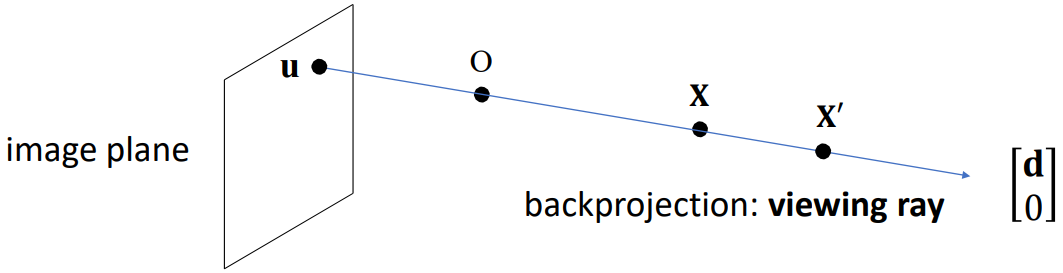
\includegraphics[width=0.6\linewidth]{images/scene.png}
    \caption{Projection from 3D scene to 2D image plane}
\end{figure}
The optical center $\mathbf{o}$ in world coordinates is: $-\mathbf{M}^{-1}\mathbf{m}$.

\subsection{Camera intrinsic parameters}
The homogeneous coordinates of an image point are represented as:
\[\mathbf{p} = \begin{bmatrix} U \\ V \\ 1 \end{bmatrix}\]

\paragraph*{Camera reference frame}
The camera reference frame is centered at the optical center $\mathbf{O}$, with the $Z$-axis perpendicular to the image plane.
The $X$ and $Y$ axes are aligned with pixel rows and columns, respectively, and distances are measured in focal length units $f$.

\paragraph*{Image reference frame}
The image reference frame is centered at the principal point $\mathbf{C}$.
The coordinates $(U, V)$ are parallel to pixel rows and columns but have an orientation opposite to the camera frame's $(X, Y)$.
Measurements along the $U$ and $V$ axes are also expressed in units of focal length $f$.

The homogeneous pixel coordinates of an image point are:
\[\mathbf{u} = \begin{bmatrix} x \\ y \\ 1 \end{bmatrix}\]
To convert between image and pixel coordinates:
\begin{itemize}
    \item A unit increment in $U$ corresponds to an increase of $fX$ pixels in $x$.
    \item A unit increment in $V$ corresponds to an increase of $fY$ pixels in $y$.
\end{itemize}
The pixel coordinates of the principal point $\mathbf{C}$ are $(U_0, V_0)$.
The relationship between pixel and image coordinates is described by the calibration matrix $\mathbf{K}$:
\[\mathbf{u} = \begin{bmatrix} x \\ y \\ 1 \end{bmatrix} = \begin{bmatrix} f_x & 0 & U_0 \\ 0 & f_y & V_0 \\ 0 & 0 & 1 \end{bmatrix} \mathbf{p}=\mathbf{K}\begin{bmatrix} \mathbf{I} & \mathbf{0}\end{bmatrix}\mathbf{X}_\text{cam}\]
Here, $\mathbf{K}$ is the intrinsic calibration matrix.

\subsection{World and camera coordinate systems}
In general, the world coordinate system is distinct from the camera coordinate system.
The transformation between world and camera coordinates is given by:
\[\mathbf{u} = \mathbf{K} \begin{bmatrix} \mathbf{R} & \mathbf{t} \\ \mathbf{0} & \mathbf{1}\end{bmatrix}\mathbf{X}_\text{world}\]
Here, $\mathbf{K}$ is the intrinsic calibration matrix, $\mathbf{R}$ is the rotation matrix, $\mathbf{t}$ is the translation vector, and $\mathbf{X}_\text{world}$ is the point in world coordinates.

The camera projection matrix $\mathbf{P}$ is then given by:
\[\mathbf{P} = \mathbf{K} \begin{bmatrix} \mathbf{R} & \mathbf{t} \end{bmatrix}\]
Thus, the projection of a world point $\mathbf{X}_\text{world}$ onto the image plane is:
\[\mathbf{u} = \mathbf{P} \mathbf{X}_\text{world} = \mathbf{K} \begin{bmatrix} \mathbf{R} & \mathbf{t} \end{bmatrix} \mathbf{X}_\text{world}\]
This can be rewritten as:
\[\mathbf{u} = \begin{bmatrix} \mathbf{M} & \mathbf{m}\end{bmatrix}    \mathbf{X}_\text{world} \]
Here, $\mathbf{M} = \mathbf{K} \mathbf{R}$ encapsulates intrinsic and rotational transformations, and $\mathbf{m} = \mathbf{K} \mathbf{t}$ represents intrinsic scaling and translation.